% FUNDAMENTAÇÃO TEÓRICA--------------------------------------------------------

\chapter{FUNDAMENTAÇÃO TEÓRICA}
\label{chap:fundamentacao-teorica}

A fundamentação teórica deste trabalho, estabelecida nas seções posteriores, evidenciará cada parte do projeto com as determinadas ferramentas e recursos os quais foram utilizados. 

\section{Análise de funcionamento e aplicação de uma cisterna}

Para desenvolvimento do trabalho, parte-se do princípio de uma estrutura previamente construída, demostrada na \autoref{fig:esquema_cisterna}. A partir dos elementos dessa figura, evidenciados na \autoref{tab:tabela_esquema_cisterna}, é possível realizar uma análise sobre o que pode ser automatizado, levando em consideração as variáveis e características do sistema.  

\begin{figure}[H]
	\centering
	\caption{Esquema de demonstração de uma cisterna no subsolo}
	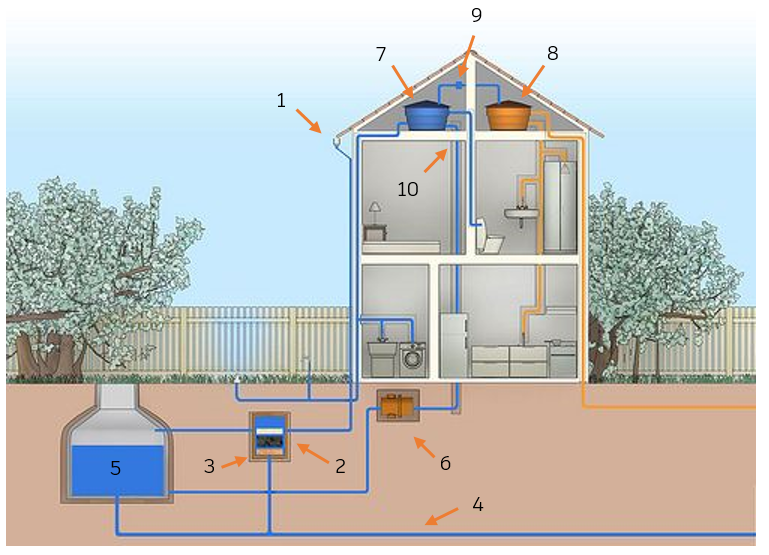
\includegraphics[width=1.0\textwidth]{figuras/esquema_cisterna.png}
	\fonte{Adaptado (ECOMONTES, 2016)}
	\label{fig:esquema_cisterna}
\end{figure} 

\newpage

\begin{table}[]
	\centering
	\small
	\begin{tabular}{c|c|c}
		\hline
		\textbf{Identificador} & \textbf{Elemento} & \textbf{Descrição} \\ \hline
		1 & Calha coletora & \begin{tabular}[c]{@{}c@{}}Elemento convencional para coleta e \\ descarte de água da chuva\end{tabular} \\ \hline
		2 & Filtro A (cascalho fino) & \begin{tabular}[c]{@{}c@{}}Elemento para realização de \\ filtragem de pequenas impurezas\end{tabular} \\ \hline
		3 & Filtro B (cascalho grosso) & \begin{tabular}[c]{@{}c@{}}Elemento para realização de \\ filtragem de impurezas\end{tabular} \\ \hline
		4 & Tubulação de descarte & \begin{tabular}[c]{@{}c@{}}Tubulação utilizada como rota de escoamento \\ quando o reservatório não está em uso ou \\ está cheio\end{tabular} \\ \hline
		5 & Reservatório de coleta & Cisterna propriamente dita \\ \hline
		6 & Motobomba ou bomda d'água & \begin{tabular}[c]{@{}c@{}}Elemento utilizado para realização do \\ ganho de elevação da água\end{tabular} \\ \hline
		7 & Caixa d'água auxiliar & \begin{tabular}[c]{@{}c@{}}Caixa d'água convencional com alimentação \\ oriunda da bomba d'água\end{tabular} \\ \hline
		8 & Caixa d'água convencional & \begin{tabular}[c]{@{}c@{}}Caixa d'água padrão com alimentação \\ da estação de água da cidade\end{tabular} \\ \hline
		9 & Elo de ligação & \begin{tabular}[c]{@{}c@{}}Ligação utilizada para abastecer a caixa d'água \\ auxiliar quando a cisterna está seca \\ ou em manutenção\end{tabular} \\ \hline
		10 & Distribuidor & \begin{tabular}[c]{@{}c@{}}Elementos de distribuição de água \\ para pontos estratégicos\end{tabular} \\ \hline
	\end{tabular}
\caption{Identificação dos elementos da \autoref{fig:esquema_cisterna}.}
\label{tab:tabela_esquema_cisterna}
\end{table}
% https://www.tablesgenerator.com

Após a evidenciar todas as características da estrutura citada anteriormente o um diagrama foi criado tendo em vista a esquematização, a organização e o esclarecimento dos requisitos.   

\begin{figure}[H]
	\centering
	\caption{Esquema básico do projeto.}
	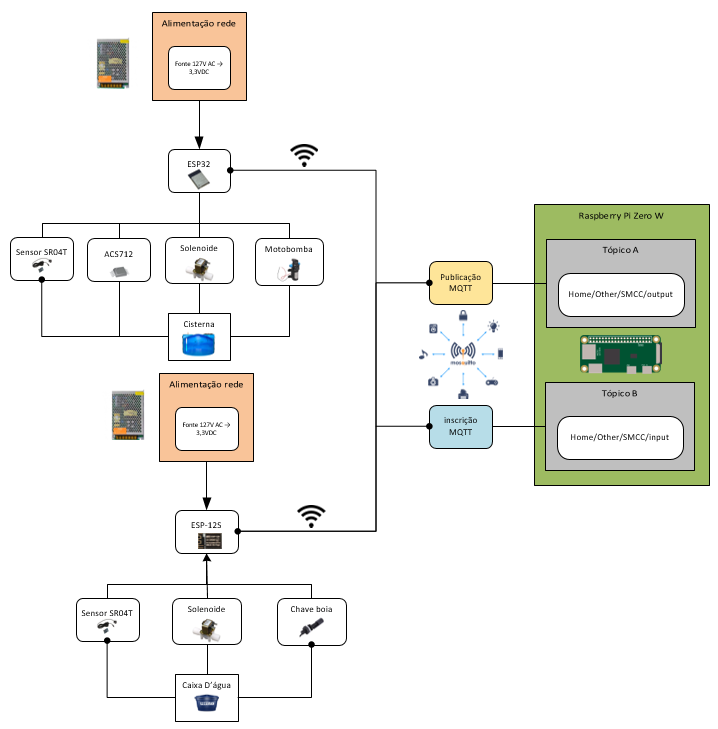
\includegraphics[width=1.0\textwidth]{figuras/esquema_basico_proj.png}
	\fonte{Própria}
	\label{fig:esp8266ex}
\end{figure} 

\section{Elementos de \textit{Hardware}}
\subsection{Os microcontroladores ESP8266 e ESP32}

O \textit{ESP8266} (\autoref{fig:esp8266ex}) é um chip microcontrolador da fabricante chinesa \textit{Espressif Systems}. Construído em torno de um processador Tensilica Xtensa LX3, inclui \textit{Wi-Fi on-board}. Originalmente concebido como um adaptador \textit{UART} para \textit{Wi-Fi} (utilizado em \textit{tablets}), permitindo que outros microcontroladores se conectem a uma rede \textit{Wi-Fi} e façam conexões \textit{TCP/IP} simples usando comandos do estilo \textit{Hayes}, o \textit{ESP8266} rapidamente se tornou popular como um microcontrolador autônomo devido ao seu ponto de preço baixo.

\begin{figure}[H]
	\centering
	\caption{\textit{ESP8266EX}.}
	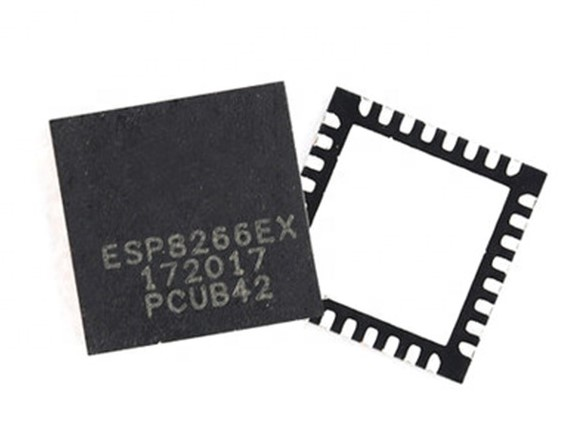
\includegraphics[width=0.3\textwidth]{figuras/esp8266ex.jpg}
	\fonte{DIGIKEY, 2020}
	\label{fig:esp8266ex}
\end{figure} 

Apesar da falta de documentação inicial, uma grande comunidade foi formada em
torno do ESP8266, e a comunidade integrou e deu suporte ao \textit{firmware} para o chip, fazendo-o compatível com a plataforma \textit{Arduino}.
Embora o chip \textit{ESP8266} seja feito pela \textit{Espressif}, existem diversos módulos criados para aplicações distintas (\autoref{fig:modulos_esp8266}).

\begin{figure}[H]
	\centering
	\caption{Alguns exemplos de módulos com base no \textit{ESP8266EX}.}
	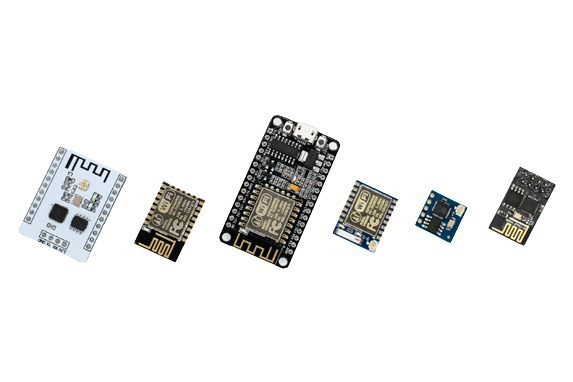
\includegraphics[width=0.5\textwidth]{figuras/modulos_esp8266.png}
	\fonte{FILIPEFLOP, 2020}
	\label{fig:modulos_esp8266}
\end{figure} 

Dentre os modelos, o \textit{ESP-12S} (\autoref{fig:esp12s}) é um módulo, baseado no microcontrolador \textit{ESP8266EX}, que será aplicado neste projeto por ser recente, externar apenas pinos utilizáveis e possuir 14 \textit{GPIOs - General Purpose Input Output} sendo ideal para a leitura de uma gama de sensores.


\begin{figure}[H]
	\centering
	\caption{Vista superior do \textit{ESP-12S}.}
	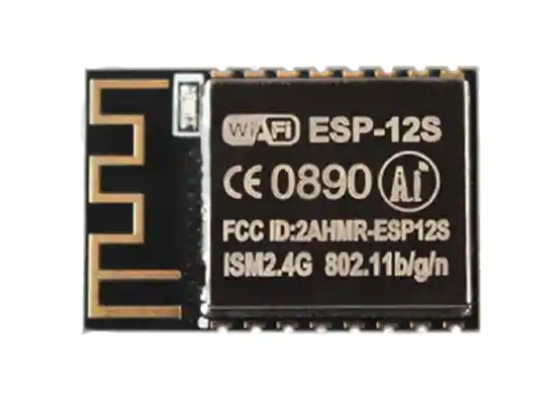
\includegraphics[width=0.3\textwidth]{figuras/ESP-12S.png}
	\fonte{FILIPEFLOP, 2020}
	\label{fig:esp12s}
\end{figure} 



O \textit{ESP32}, apresentado na \autoref{fig:esp32}, é um \textit{chip} também desenvolvido pela \textit{Espressif Systems}. Ele fornece além da conectividade \textit{Wi-Fi}, também presente no \textit{ESP8266}, a possibilidade de conexão \textit{Bluetooth}. Possuindo também uma maior \textit{perfomance} em âmbitos de processamento (dois núcleos), o \textit{ESP32} fornece uma maior quantidade de \textit{GPIOs}, que totalizam 34.  Embora o dispositivo seja tecnicamente apenas o \textit{chip}, existem também diversos módulos fabricados por empresas para aplicações específicas que carregam o nome "\textit{ESP32}", como o da figura abaixo.

\begin{figure}[H]
	\centering
	\caption{Vista superior do \textit{ESP32}.}
	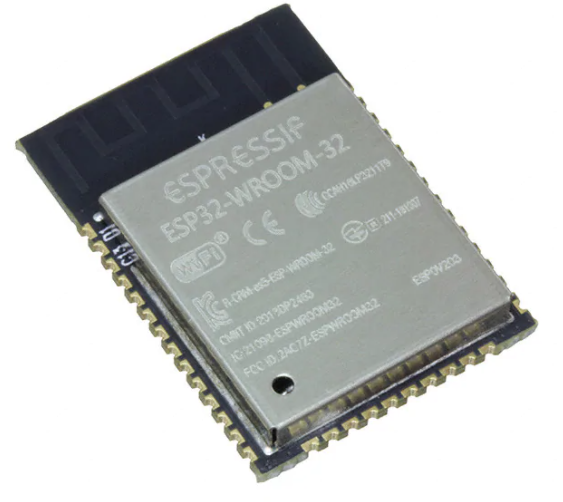
\includegraphics[width=0.3\textwidth]{figuras/ESP32.png}
	\fonte{DIGIKEY, 2020}
	\label{fig:esp32}
\end{figure} 

\subsection{A Raspberry Pi Zero W}

A \textit{Raspberry Pi Zero W} é basicamente um computador de placa única. Ela possui recursos como \textit{slot} para cartão \textit{microSD}, conectores \textit{HDMI} e de câmera, conectividade \textit{Wi-Fi} e \textit{Bluetooth 4.0}, um conector macho de entrada-saída (\textit{GPIO}) de 40 pinos e mini conector de alimentação \textit{+ 5VDC}. O microcontrolador baseado no processador \textit{BCM2835 ARMv7 system-on-chip (SoC)} alimenta o Pi Zero W.

Essa versão de \textit{Hardware} é muito compacta, ficando no meio termo entre as fazes de prototipação e aplicação. Com o microprocessador \textit{ARM BCM2835} de \textit{1GHz}, memória \textit{RAM} de \textit{512MB} e um sistema operacional enxuto instalado, a Raspberry Pi Zero W é ideal para rodar aplicações como um \textit{Broker MQTT}.

\begin{figure}[H]
	\centering
	\caption{Vista superior da \textit{Raspberry Pi Zero W}}
	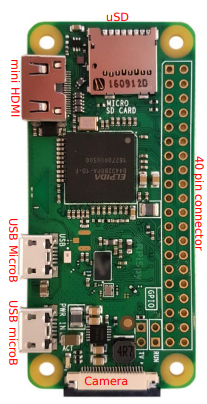
\includegraphics[width=0.3\textwidth, angle = 90]{figuras/rasp_zerow.png}
	\fonte{SPARKFUN, 2020}
	\label{fig:rasppizerow}
\end{figure} 

\subsection{A fonte de alimentação DC}

Para alimentação elétrica de todos os dispositivos eletrônicos envolvidos no processo de automação da cisterna, a fonte chaveada \textit{12V/10A} representada na \autoref{fig:fontechaveada}, é ideal por possuir características robustas, como proteção mecânica e eletrônica. Esse tipo de fonte também disponibiliza vários conectores de saída, os quais podem ser interligados para pontos específicos de alimentação.

\begin{figure}[H]
	\centering
	\caption{Vista superior da fonte}
	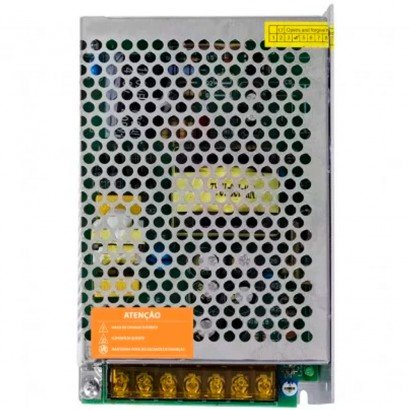
\includegraphics[width=0.4\textwidth]{figuras/fonte_chaveada.jpg}
	\fonte{AMAZON, 2020}
	\label{fig:fontechaveada}
\end{figure} 

\subsection{A motobomba ou bomba d'água}

A bomda d'água selecionada, \autoref{fig:bomba} , trabalha com fontes de alimentação de correntes contínuas (\textit{DC}) o que permite um maior controle do funcionamento através de sistemas \textit{microprocessados}. Essa bomba opera a \textit{12V}, com potência máxima de \textit{80W}. Ela possui a capacidade de exercer uma vazão de \textit{5,5L/min} com ganho de elevação de no máximo \textit{40m}.

\begin{figure}[H]
	\centering
	\caption{Bomda d'água \textit{DC}}
	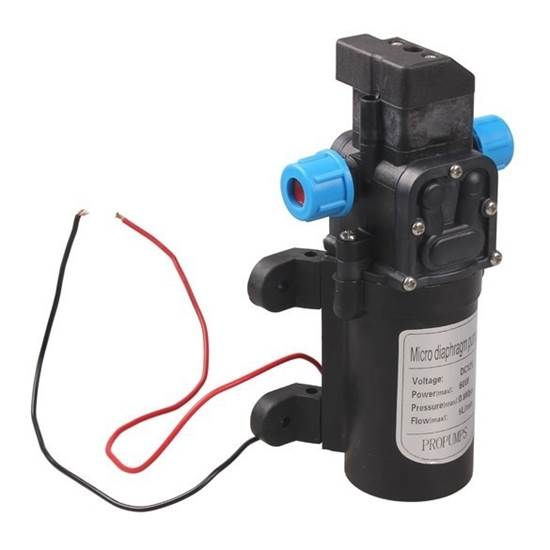
\includegraphics[width=0.3\textwidth]{figuras/bomba.jpeg}
	\fonte{ENERGIA TOTAL, 2020}
	\label{fig:bomba}
\end{figure} 


\subsection{O sensor de corrente}

O sensor de corrente ACS712 selecionado é barato e oferece precisão em
soluções para detecção de corrente AC ou DC na indústria,
comercial e sistemas de comunicação. O dispositivo permite fácil implementação: aplicações típicas incluem controle de motor, detecção de carga e
gerenciamento, fontes de alimentação comutadas e sobrecorrente
proteção contra falhas.


\begin{figure}[H]
	\centering
	\caption{Representação gráfica do sensor \textit{ACS712}}
	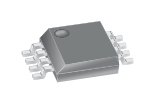
\includegraphics[width=0.3\textwidth]{figuras/ACS712.png}
	\fonte{ALEGRO, 2020}
	\label{fig:acs712}
\end{figure} 


O dispositivo consiste em um operador \textit{Hall} linear preciso, a corrente aplicada flui através do material de cobre gerando um campo magnético que é detectado pelo \textit{Hall} integrado e convertido em um proporcional de tensão. A precisão do dispositivo é otimizada por meio do fechamento proximidade do sinal magnético ao transdutor \textit{Hall}. A resistência interna do material condutor atinge uma méddia de \textit{1,2m}$\Omega$, proporcionando baixa potência. De acordo \textit{datasheet} do componente, pode-se observar a simples aplicação típica representada na figura abaixo.
 
\begin{figure}[H]
	\centering
	\caption{Aplicação típica do\textit{ACS712}}
	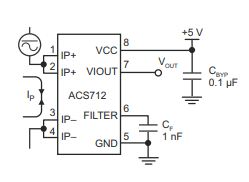
\includegraphics[width=0.4\textwidth]{figuras/ACS712_typical.png}
	\fonte{ALEGRO, 2020}
	\label{fig:acs712_typical}
\end{figure} 

\subsection{Os elementos de ativação e desativação}

Tendo em vista os elementos descritos nos itens anteriores, tornou-se necessário a implementação de um circuito para ativação e desativação da bomba d'água assim como a execução de técnicas de proteção e isolamento.

O diagrama desenvolvido no \textit{software Proteus} (\autoref{fig:diagramaproteus}) mostra a integração de como seria o sistema de ativação e desativação da motobomba.

\begin{figure}[H]
	\centering
	\caption{Diagrama de ativação com partida lenta}
	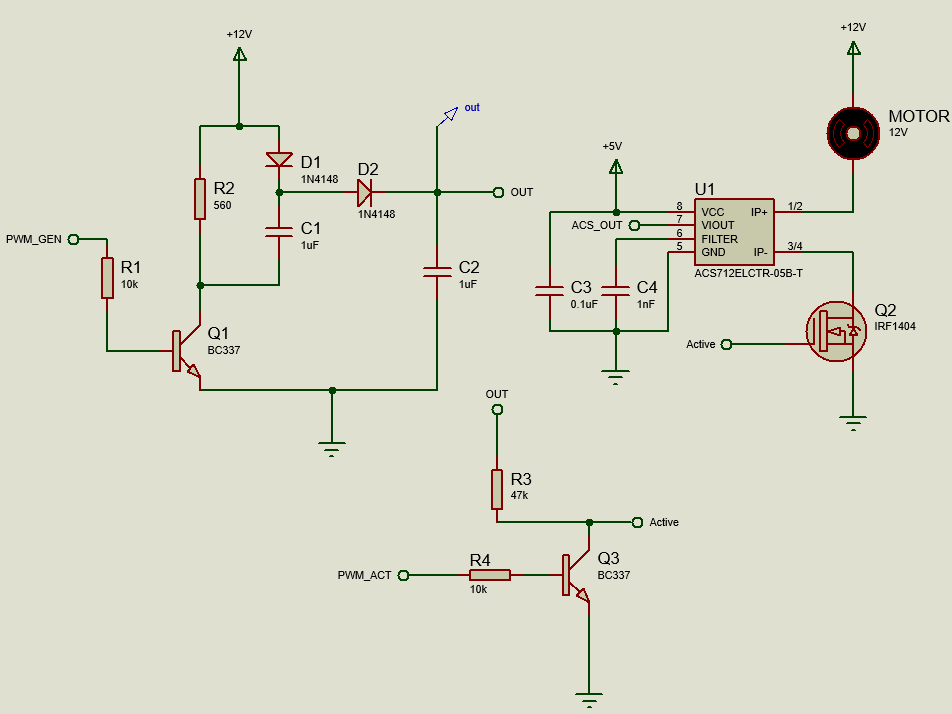
\includegraphics[width=0.9\textwidth]{figuras/diagrama_ativação_bomba.png}
	\fonte{Própria}
	\label{fig:diagramaproteus}
\end{figure} 

A partir deste diagrama utilizou-se técnicas de partida lenta através do chaveamento transistorizado (\textit{BC337}). Por meio do \textit{PWM - Pulse-Width Modulation} oriundo do microcontrolador, o transistor realiza a alteração sobre o valor eficaz de tensão aplicada na bomba d'água.

Para saturação do transistor \textit{IRF1404} (\autoref{fig:IRF1404}) foi desenvolvido o circuito dobrador de tensão também evidenciado na \autoref{fig:diagramaproteus}. A ideia desse circuito é garantir uma queda de tensão entre \textit{GATE} e \textit{SOURCE} duas vezes maior (em torno de \textit{24V}) que a tensão de alimentação do circuito.

\begin{figure}[H]
	\centering
	\caption{Transistor IRF1404}
	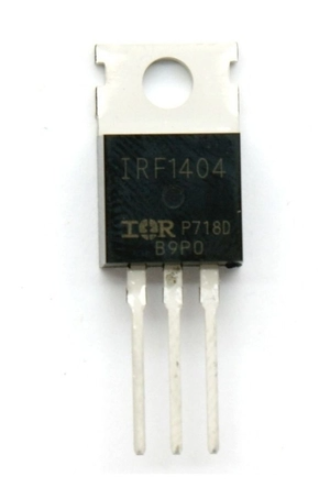
\includegraphics[width=0.2\textwidth]{figuras/IRF1404.png}
	\fonte{ALLDATASHEET, 2020}
	\label{fig:IRF1404}
\end{figure} 

\subsection{O sensor de distância ultrassônico}
\label{ssec:sensor_ultra}
O Sensor Ultrassônico de Distância selecionado foi o \textit{JSN-SR04T}, desenvolvido exclusivamente para aperfeiçoar projetos de robótica e microeletrônica, mostrando-se capaz de medir distâncias, em relação a objetos, na faixa entre \textit{25cm} à \textit{150cm}.

\begin{figure}[H]
	\centering
	\caption{Sensor ultrassônico \textit{JSN-SR04T} e módulo de conversão}
	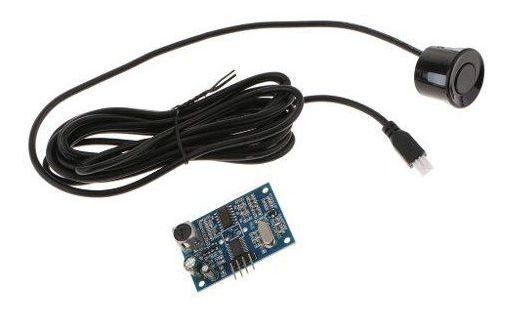
\includegraphics[width=0.5\textwidth]{figuras/sensor_ultra.jpg}
	\fonte{USINAINFO, 2020}
	\label{fig:sensor_ultra}
\end{figure}

O ponto interessante desse sensor é sua ampla e eficiente resistência à umidade, sendo principalmente utilizado em ambientes úmidos, permitindo manter ampla distância do microcontrolador. Ele possui com um fio de \textit{2,5 metros} de comprimento e um módulo especialmente desenvolvido para atuar em conjunto com microcontroladores necessitando de apenas quatro portas de conexão: \textit{5V} (VCC), \textit{Trig (RX)}, \textit{Echo (TX)} e \textit{GND}.

O funcionamento é simples, o sensor emite sinais ultrassônicos que são refletidos ao atingirem determinado objeto. Esses sinais refletidos retornam ao sensor e são processados, tomando como base o tempo de emissão e recepção através do módulo. Em pesquisas realizadas esse sensor apresentou-se ser muito eficiente para a realização da medição de nível.

\subsection{A válvula solenoide}

 O modelo de válvula solenoide selecionado possui características como:  \textit{1/2"} x \textit{1/2"}, tensão de operação em torno de \textit{12V} e consumo médio, quando ativada, de \textit{120mA}. Possui o objetivo de controlar o fluxo de água por meio de comandos elétricos e pode ser utilizada em sistemas de irrigação, tratamento de água ou em qualquer projeto que necessite de um controle sobre o fluxo de líquidos. Essa válvula em seu estado desenergizado impede o fluxo de líquido (NF - Normalmente Fechada), isso garante que durante a eventual falta de energia o líquido se manterá contido.
 
 \begin{figure}[H]
 	\centering
 	\caption{Válvula solenoide}
 	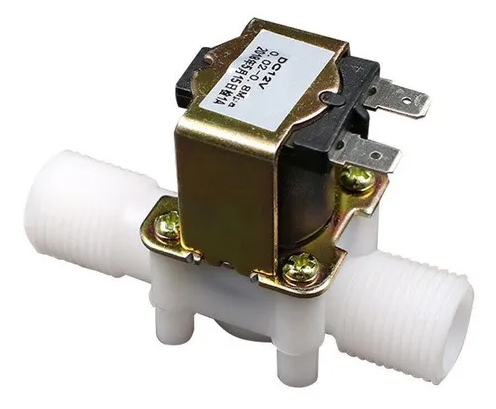
\includegraphics[width=0.4\textwidth]{figuras/solenoide.png}
 	\fonte{SMART KITS, 2020}
 	\label{fig:solenoide}
 \end{figure}

\subsection{A chave de nível tipo boia}

Para questões de segurança a chave de nível \textit{RF-0H21D} será utilizada para fomentar a redundância do sistema, caso aconteçam falhas na medição do sensor citado na seção \ref{ssec:sensor_ultra}. Essa chave indicará para o microcontrolador, por meio de contato elétrico, o momento exato para desativação da bomba d'água, evitando possíveis vazamentos. 

 \begin{figure}[H]
	\centering
	\caption{Chave de nível \textit{RF-0H21D}}
	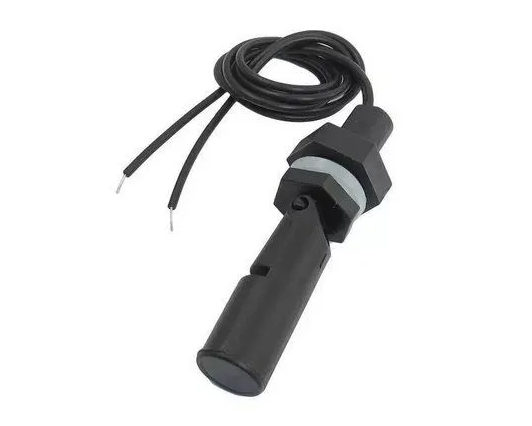
\includegraphics[width=0.5\textwidth]{figuras/chave_boia.png}
	\fonte{SMART KITS, 2020}
	\label{fig:chaveboia}
\end{figure}


\section{Elementos de \textit{Firmware}}
\subsection{O Ambiente de Desenvolvimento Integrado \textit{Arduino}}

A plataforma Arduino, criada em 2005, não abrange somente as placas microcontroladas mas também agrega-se de uma Interface de Desenvolvimento, ou seja uma IDE, que possui um compilador \textit{C++}. A utilização dessa IDE se tornou tão difundida atualmente que grandes empresas de tecnologia têm buscado tornar ou fabricar microcontroladores completamente compatíveis com a interface.  
Com esta interface, será possível a programação dos microcontroladores \textit{ESP8266} e \textit{ESP32} de maneira facilitada e sem a necessidade do aprendizado de uma nova liguagem. Todas as funcionalidades, como rotinas de conexão \textit{HTTP} e/ou \textit{MQTT} através do \textit{Wi-Fi}, Interrupção, Timers, Modos de Energia são completamente acessíveis. 

\begin{figure}[H]
	\centering
	\caption{Gerenciador de placas com suporte oficial às placas \textit{ESP32} e \textit{ESP8266}}
	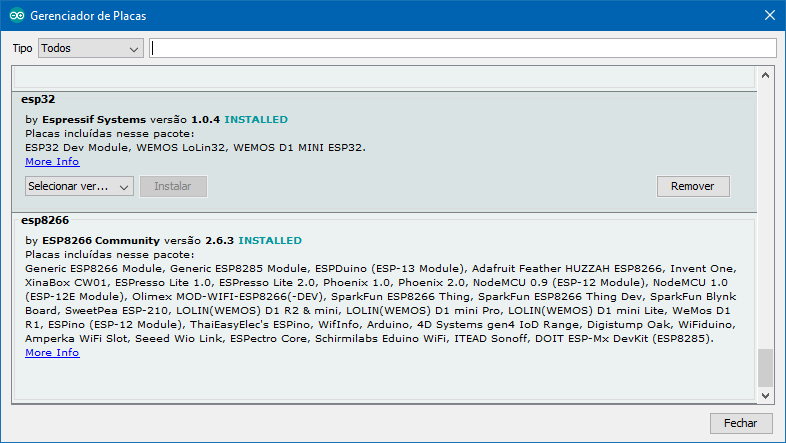
\includegraphics[width=1.0\textwidth]{figuras/gerenciador_placas_arduino.png}
	\fonte{Própria}
	\label{fig:youcto-fluxo}
\end{figure} 

\subsection{Modelagem de um \textit{SO} embarcado com \textit{Yocto Project}}

O \textit{Yocto Project} é um projeto colaborativo de código aberto que fornece modelos, ferramentas e métodos facilitando a criação de sistemas personalizados baseados em Linux para implantações de sistemas embarcados em dispositivos conectados, servidores ou ambientes virtuais, independentemente da arquitetura de hardware.

Por ser um projeto \textit{open source}, opera com uma estrutura de governança hierárquica baseada na meritocracia e gerenciada por seu arquiteto-chefe. Isso permite que o projeto permaneça independente de qualquer um de seus organizadores membros, que participam de várias maneiras e fornecem recursos para o projeto.

O projeto é apoiado e administrado por líderes da indústria de alta tecnologia que se comprometeram financeiramente, com suporte de plataforma e esforços de marketing para tornar o \textit{Yocto Project} um padrão seguro, estável e adaptável da indústria.

\begin{figure}[H]
	\centering
	\caption{Fluxo de trabalho geral \textit{Yocto Project}}
	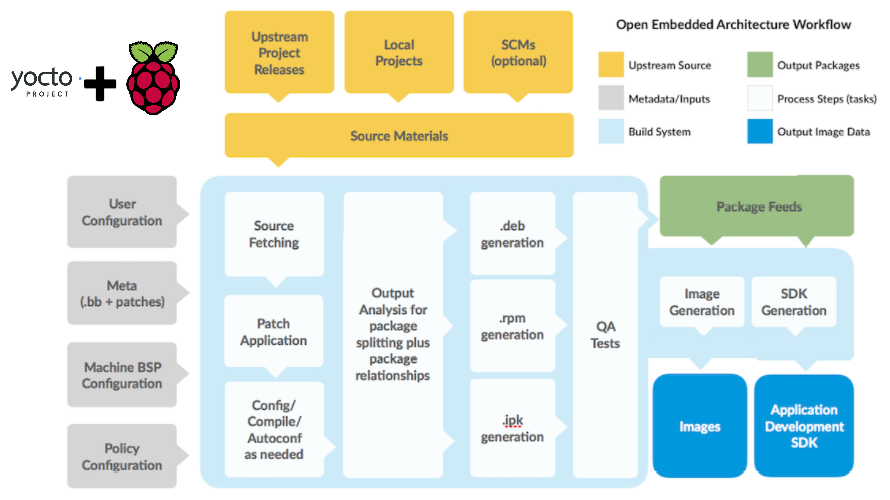
\includegraphics[width=1.0\textwidth]{figuras/yocto-fluxo.png}
	\fonte{Adaptado (yoctoproject.org, 2020)}
	\label{fig:youcto-fluxo}
\end{figure} 

\section{Elementos de \textit{Software}}
\subsection{O \textit{framework React Native}}

Baseado no \textit{React}, para desenvolvimento \textit{WEB}, o \textit{React Native} é um \textit{framework} de codigo aberto desenvolvido pela equipe do \textit{Facebook} que suporta a criação de aplicativos \textit{mobile} multiplataforma (Android e iOS), sem que haja a preocupação de lidar com as linguagens padrões como \textit{Java} ou \textit{Swift}, usando apenas \textit{Javascript}. Como ponto positivo, ao contrário de outros \textit{frameworks} com o mesmo propósito, todo código desenvolvido com \textit{React Native} será convertido para a linguagem nativa do sistema operacional, o que torna o aplicativo mais performático.

\begin{figure}[H]
	\centering
	\caption{Exemplos de \textit{Templates} produzidos com \textit{React Native}}
	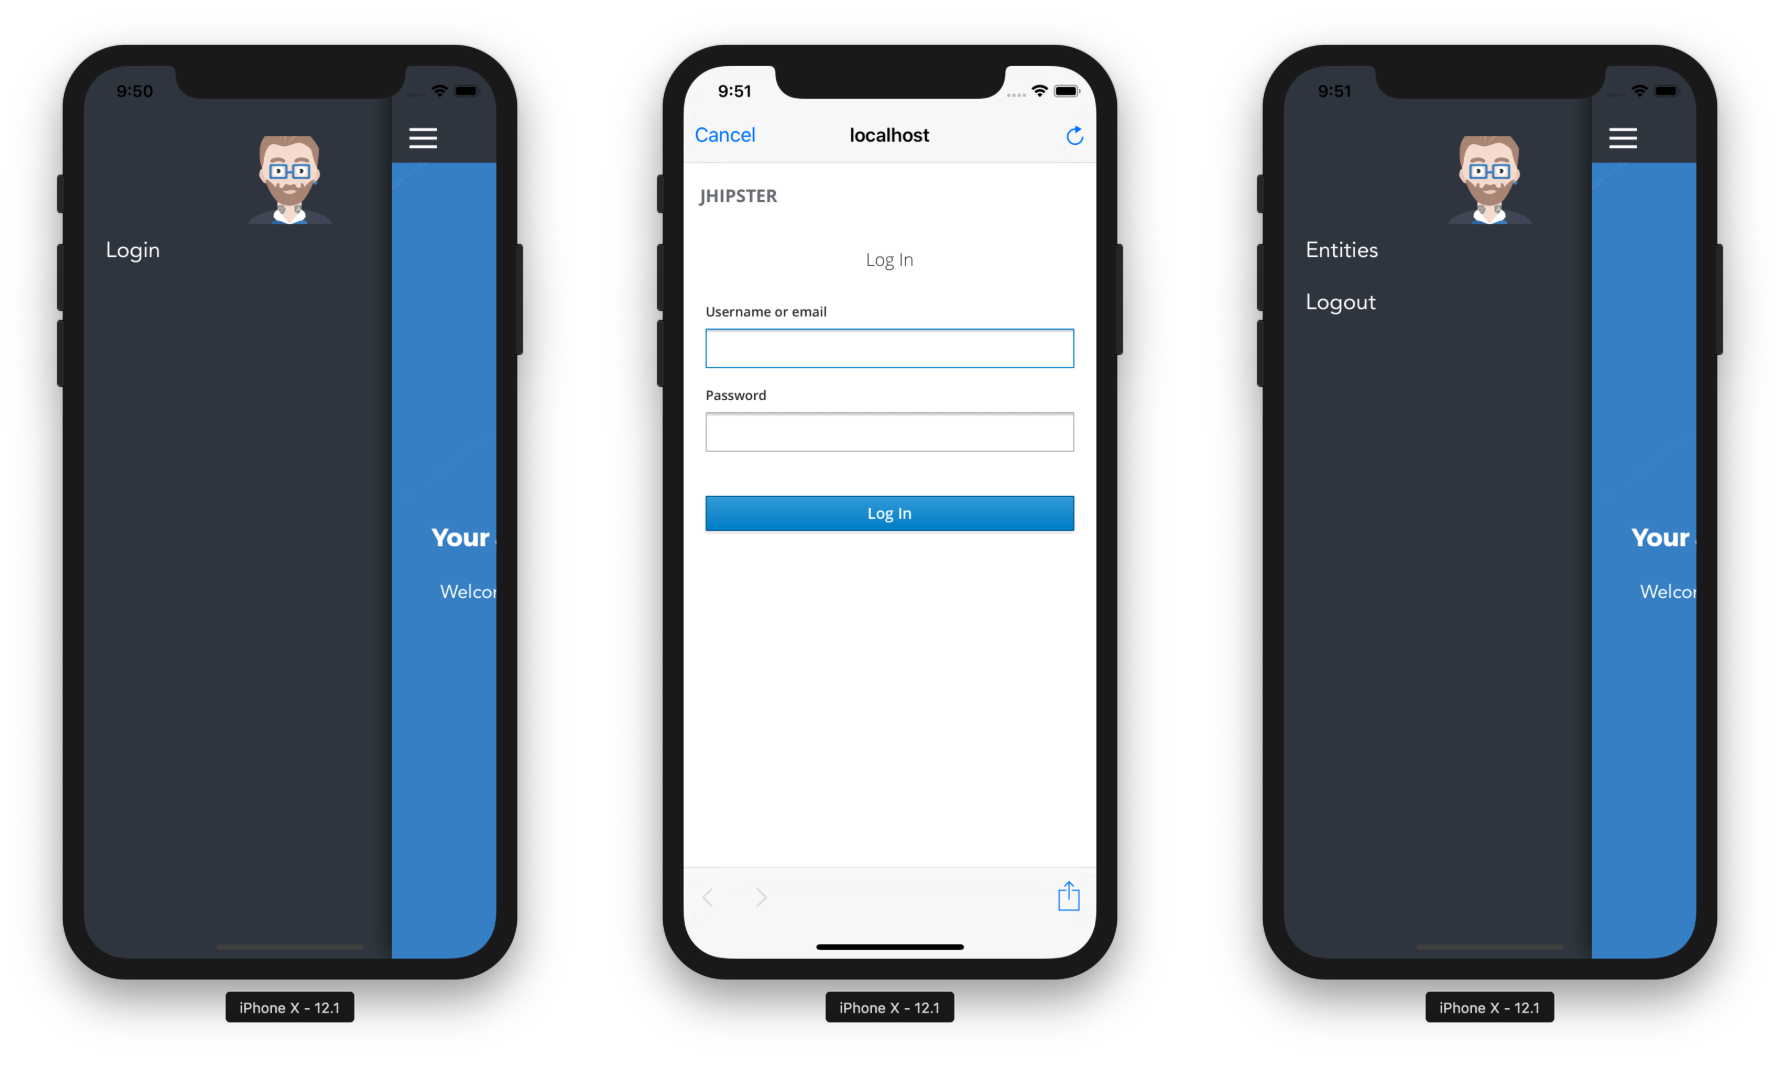
\includegraphics[width=0.7\textwidth]{figuras/react_native_elements.png}
	\fonte{Adaptado (instamobile.io, 2020)}
	\label{fig:youcto-fluxo}
\end{figure} 

\subsection{O \textit{framework Electron}}

O \textit{Electron} é um \textit{framework} multiplataforma (Windows, Linux e MacOS) para criação de interfaces possibilitando o usuário acessar serviços do sistema operacional tanto via linha de comando - \textit{CLI} e interface gráfica - \textit{GUI}.

\begin{figure}[H]
	\centering
	\caption{Aplicações que utilizam \textit{Electron}}
	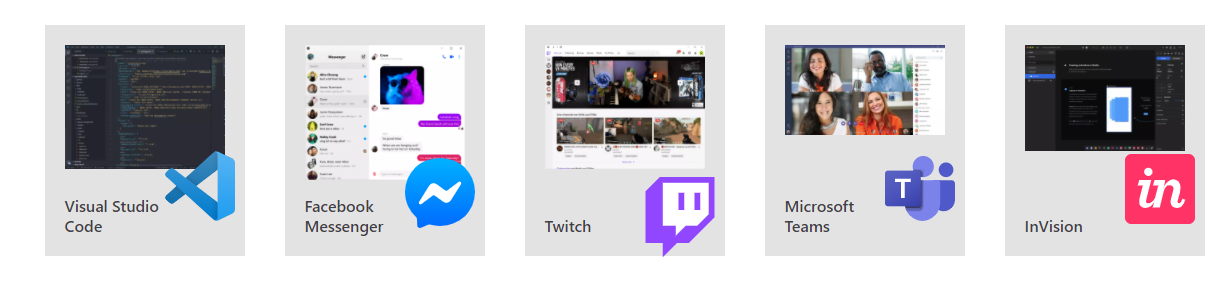
\includegraphics[width=1.0\textwidth]{figuras/electron_apps.png}
	\fonte{Adaptado (electronjs.org, 2020)}
	\label{fig:youcto-fluxo}
\end{figure} 

Por meio dele podemos desenvolver aplicações \textit{desktop} utilizando \textit{HTML}, \textit{CSS} e \textit{Javascript}. O \textit{Electron} vem com navegador \textit{Chromium}, um projeto \textit{open source} de onde surgiu o \textit{Google Chrome}. Toda a parte visual, janelas, etc. são renderizadas nessa camada e o \textit{BackEnd} é executado em \textit{Node.js}. Ambos tem acesso um ao outro via RPC (Remote Procedure Call).



